\section{PS6: Random Writer}\label{sec:ps6}

\subsection{Discussion}\label{sec:ps6:disc}

This program takes a string and two integers. one of the integer decides how many characters the map is going to store from the string. Then, interacts with the map to randomly produce a character or a string.

\begin{figure}[tbh]
	\centering
	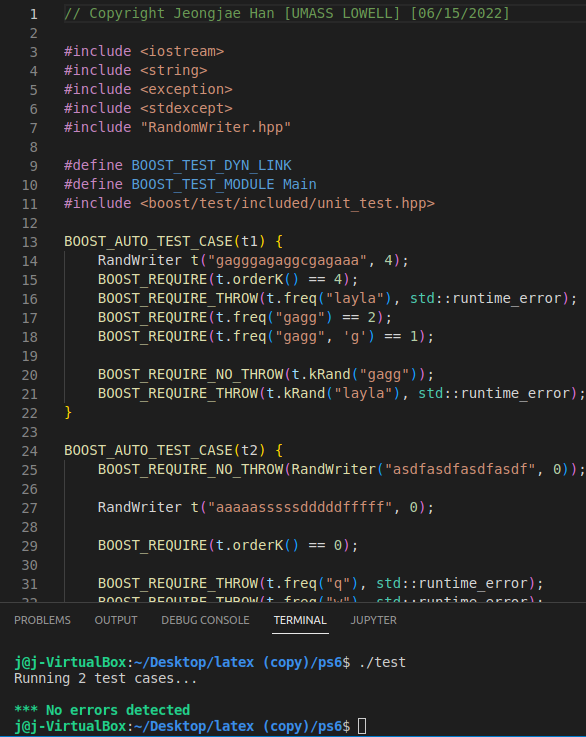
\includegraphics[width=8cm]{ps6_test}
	\caption{Testing ps6 codes}
	\label{fig:ps6_test}
\end{figure}

My test has no error.
I made two tests. My test.cpp file tests all the public functions, and exception, but generate function because I am not sure how to make a test for a generate which generates a random string that I cannot even predict the result.

\begin{figure}[tbh]
	\centering
	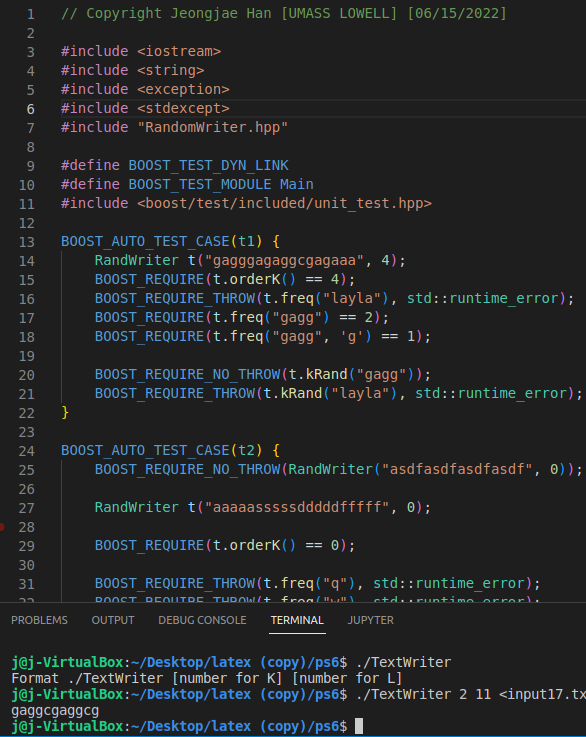
\includegraphics[width=8cm]{ps6}
	\caption{Testing ps6 codes}
	\label{fig:ps6}
\end{figure}

I was not sure about input17.txt, so I created input17.txt and it has example string that the prompt provided.

I tried to use size-t for index for for-loops because we covered it in during the class.

Also, for iterator, I used auto p instead of ::iterator p and for-each loop because the map was declared as private member of the class, so the compiler was asking for operator functions.

\subsection{Places to get help}
I got help from Youtube, Comp3 assignments, stackoverflow, c++reference, how to loop through a map.pdf.

%\subsection{What I accomplished}\label{sec:ps0:accomplish}

%\subsection{What I already knew}\label{sec:ps0:knew}

\subsection{What I learned}\label{sec:ps6:learned}

I learned how I should interact with a map. For comp3, there was an assignment that I have to use map, and it helped me to get to know about map, but this project helped me to get used to it. I also referred the assignment for this project.

\subsection{Mistakes}\label{sec:ps6:Mistakes}
I got three points off.
I could not use lambda expression as parameter for this project, I tried to use it in the kRand. I made a random function by using lambda expression and declaring a variable as auto, but I am not sure if this is working as a parameter.
My kRand did not generate all expected characters.
Also, my output was not reasonable.

\subsection{Codebase}\label{sec:ps6:code}
Makefile
\lstinputlisting[language=Make]{ps6/Makefile}
TextWriter.cpp
\lstinputlisting{ps6/TextWriter.cpp}
RandomWriter.hpp
\lstinputlisting{ps6/RandomWriter.hpp}
RandomWriter.cpp
\lstinputlisting{ps6/RandomWriter.cpp}
test.cpp
\lstinputlisting{ps6/test.cpp}

\newpage
